\documentclass[aspectratio=169,11pt]{beamer}

% ==================== THÈME ET ESTHÉTIQUE ====================
\usetheme{Madrid}
\usecolortheme{seahorse}
\setbeamertemplate{navigation symbols}{}
\setbeamertemplate{footline}[frame number]
\setbeamertemplate{frametitle}[default][center]

% Couleurs personnalisées élégantes
\definecolor{mainblue}{RGB}{45, 62, 80}
\definecolor{accentorange}{RGB}{211, 84, 0}
\definecolor{lightgray}{RGB}{236, 240, 241}
\definecolor{darktext}{RGB}{44, 62, 80}

\setbeamercolor{title}{fg=mainblue}
\setbeamercolor{frametitle}{fg=white,bg=mainblue}
\setbeamercolor{structure}{fg=mainblue}
\setbeamercolor{block title}{bg=mainblue,fg=white}
\setbeamercolor{block body}{bg=lightgray,fg=darktext}
\setbeamercolor{block title alerted}{bg=accentorange,fg=white}
\setbeamercolor{block body alerted}{bg=lightgray,fg=darktext}

% ==================== PACKAGES ====================
\usepackage[utf8]{inputenc}
\usepackage[T1]{fontenc}
\usepackage[french]{babel}
\usepackage{graphicx}
\usepackage{booktabs}
\usepackage{tikz}
\usetikzlibrary{shapes.geometric, arrows, positioning, calc}
\usepackage{xcolor}
\usepackage{colortbl}

\graphicspath{{images/}}

% ==================== INFORMATIONS ====================
\title[Prédiction RUL CMAPSS]{\textbf{Prédiction Data-Driven de la Vie Utile Résiduelle}}
\subtitle{Application au jeu de données CMAPSS de la NASA}
\author[Votre Nom]{\textbf{[Votre Prénom Nom]}}
\institute[École d'Ingénieurs]{École d'Ingénieurs -- Projet de Fin de Module}
\date{2025--2026}

% ==================== DÉBUT DU DOCUMENT ====================
\begin{document}

% ----------------------------------------------------
\begin{frame}[plain]
\titlepage
\end{frame}

% ----------------------------------------------------
\begin{frame}{Plan de la présentation}
\tableofcontents
\end{frame}

% ==================== INTRODUCTION ====================
\section{Introduction}

\begin{frame}{Contexte et motivation}
\begin{columns}[T]
\begin{column}{0.55\textwidth}
\textbf{Maintenance prédictive :}
\begin{itemize}
    \item Anticiper les défaillances avant qu'elles ne surviennent
    \item Minimiser les arrêts de production imprévus
    \item Optimiser la planification des interventions
\end{itemize}
\vspace{0.3cm}
\textbf{Problématique :} Comment prédire la \textcolor{accentorange}{\textbf{Vie Utile Résiduelle}} (RUL) d'un moteur turbofan à partir de données capteurs ?
\end{column}
\begin{column}{0.42\textwidth}
\begin{block}{Définition -- RUL}
Nombre d'unités de temps restantes avant qu'un composant ne puisse plus accomplir sa fonction désirée.
\end{block}
\end{column}
\end{columns}
\end{frame}

\begin{frame}{Objectifs du projet}
\begin{enumerate}
    \item \textbf{Explorer} le jeu de données public CMAPSS (NASA)
    \item \textbf{Prétraiter} les données temporelles de dégradation de moteurs
    \item \textbf{Implémenter} et comparer deux approches data-driven :
    \begin{itemize}
        \item \textbf{XGBoost} -- Gradient boosting (machine learning classique)
        \item \textbf{LSTM} -- Réseaux de neurones récurrents profonds
    \end{itemize}
    \item \textbf{Évaluer} quantitativement les performances (RMSE, S-score)
    \item \textbf{Démontrer} via une interface Streamlit interactive
\end{enumerate}
\end{frame}

% ==================== DONNÉES ====================
\section{Jeu de données et prétraitement}

\begin{frame}{CMAPSS -- Commercial Modular Aero-Propulsion System Simulation}
\begin{columns}[T]
\begin{column}{0.50\textwidth}
\textbf{Origine :} NASA Prognostics Center of Excellence
\vspace{0.2cm}

\textbf{Données FD001 :}
\begin{itemize}
    \item 100 moteurs turbofan simulés
    \item 26 colonnes par observation
    \item Fichiers : train, test, RUL (vérité terrain)
\end{itemize}
\vspace{0.2cm}
\textbf{Structure :}
\begin{itemize}
    \item Col 1--2 : ID moteur, cycle
    \item Col 3--5 : Réglages opérationnels
    \item Col 6--26 : 21 capteurs
\end{itemize}
\end{column}
\begin{column}{0.48\textwidth}
\begin{block}{Tâche de prédiction}
\centering
\texttt{train} : cycles jusqu'à défaillance\\[0.2cm]
\texttt{test} : cycles partiels\\[0.2cm]
\texttt{RUL} : vérité terrain\\[0.2cm]
\textbf{Objectif :} Prédire la RUL pour chaque moteur test
\end{block}
\end{column}
\end{columns}
\end{frame}

\begin{frame}{Analyse exploratoire -- Capteurs}
\begin{center}
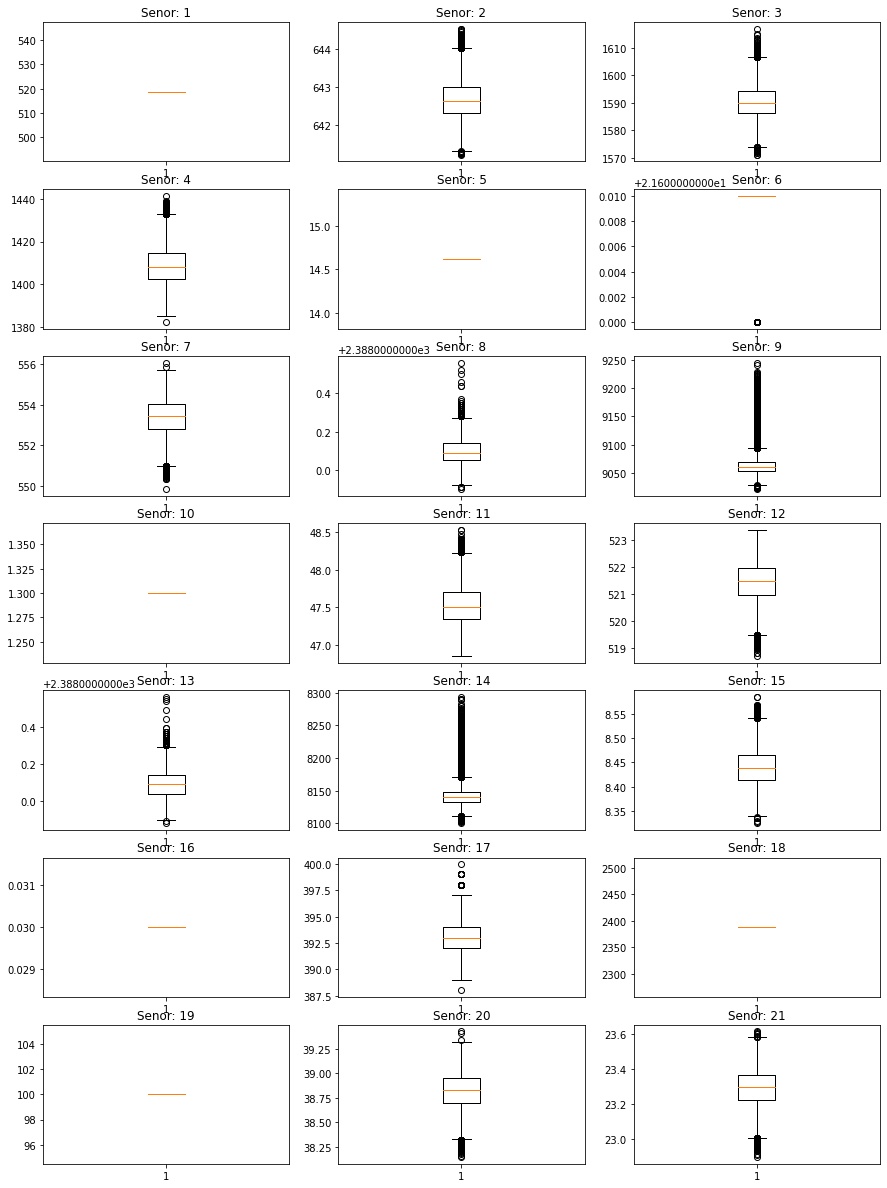
\includegraphics[height=0.62\textheight]{preprocessing_cell27_out0.png}
\end{center}
\vspace{-0.15cm}
\begin{itemize}
    \item 21 capteurs analysés via diagrammes en boîte
    \item Certains capteurs présentent une variance quasi nulle
\end{itemize}
\end{frame}

\begin{frame}{Sélection des capteurs pertinents}
\begin{columns}[T]
\begin{column}{0.48\textwidth}
\textbf{Capteurs écartés (constants) :}
\begin{itemize}
    \item Colonne 6, 10, 15, 21, 23, 24
    \item Colonne 11 (quasi-constant : 21.60 / 21.61)
\end{itemize}
\vspace{0.3cm}
\textbf{Capteurs retenus :} \textcolor{accentorange}{\textbf{14 capteurs}}

\vspace{0.3cm}
\textbf{Normalisation :} MinMaxScaler avec plage [-1, 1] appliquée \emph{moteur par moteur}
\end{column}
\begin{column}{0.50\textwidth}
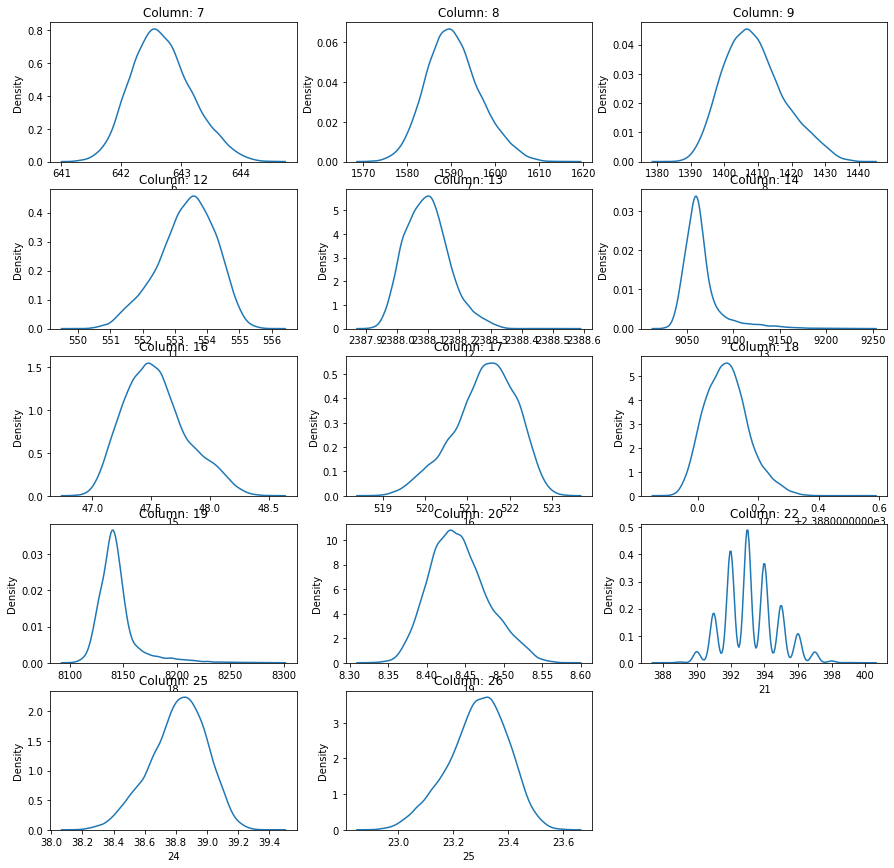
\includegraphics[height=0.55\textheight]{preprocessing_cell31_out0.png}
\end{column}
\end{columns}
\end{frame}

\begin{frame}{Similarité train / test}
\begin{center}
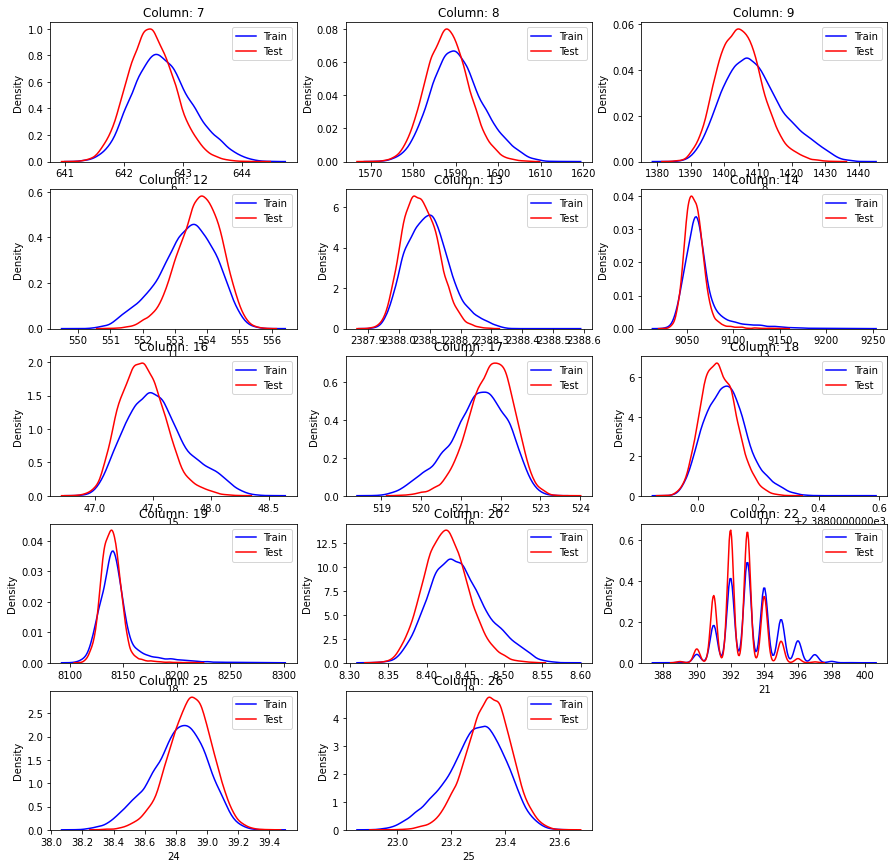
\includegraphics[height=0.58\textheight]{preprocessing_cell33_out0.png}
\end{center}
\vspace{-0.1cm}
\begin{block}{Constat}
Les distributions des données de test (orange) sont globalement similaires à celles d'entraînement (bleu) -- condition favorable à la généralisation.
\end{block}
\end{frame}

\begin{frame}{Modélisation de la dégradation}
\begin{columns}[T]
\begin{column}{0.48\textwidth}
\textbf{Modèle linéaire :}

La RUL diminue d'un cycle à chaque étape jusqu'à atteindre zéro.
\vspace{0.4cm}

\textbf{Modèle linéaire par morceaux :}

La RUL est plafonnée à une valeur maximale (early RUL = 125 cycles) tant que le moteur est récent, puis décroît linéairement.
\vspace{0.2cm}
Cette approche est largement utilisée dans la littérature pour améliorer la précision des prédictions.
\end{column}
\begin{column}{0.50\textwidth}
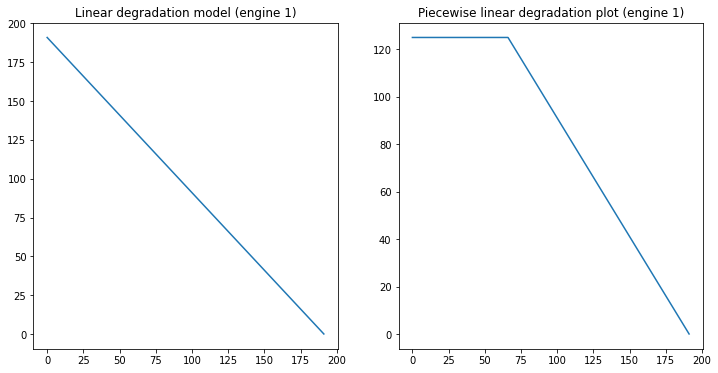
\includegraphics[width=\textwidth]{preprocessing_cell11_out0.png}
\end{column}
\end{columns}
\end{frame}

\begin{frame}{Fenêtrage temporel des séquences}
\begin{columns}[T]
\begin{column}{0.50\textwidth}
\textbf{Principe :} Extraire des fenêtres glissantes de longueur 30 cycles avec un chevauchement maximal (décalage de 1 cycle).
\vspace{0.3cm}

\textbf{Forme des tenseurs :}
\begin{itemize}
    \item Entrée : dimensions (B, 30, 14)
    \item B = nombre total de fenêtres générées
    \item 30 cycles d'historique
    \item 14 capteurs
\end{itemize}
\vspace{0.3cm}
\textbf{Prédiction test :} Moyenne des prédictions sur les N dernières fenêtres de chaque moteur.
\end{column}
\begin{column}{0.48\textwidth}
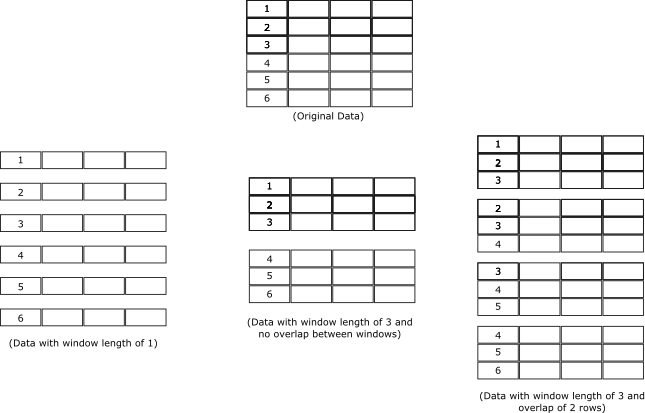
\includegraphics[width=\textwidth]{data_windowing_prognosis.png}
\end{column}
\end{columns}
\end{frame}

% ==================== MÉTRIQUES ====================
\section{Métriques d'évaluation}

\begin{frame}{RMSE et S-score}
\begin{columns}[T]
\begin{column}{0.48\textwidth}
\begin{block}{RMSE (Root Mean Square Error)}
\centering
Racine carrée de la moyenne des carrés des écarts entre la RUL réelle et la RUL prédite.
\vspace{0.1cm}

Métrique principale -- pénalise les grandes erreurs.
\end{block}
\end{column}
\begin{column}{0.48\textwidth}
\begin{alertblock}{S-score (asymétrique)}
\centering
Somme de pénalités appliquées à chaque moteur.

Les surestimations (prédire une RUL trop élevée) sont pénalisées bien plus fortement que les sous-estimations.
\vspace{0.1cm}

Pénalise plus les \textbf{surestimations} (risque de défaillance imprévue).
\end{alertblock}
\end{column}
\end{columns}
\end{frame}

% ==================== XGBOOST ====================
\section{Modèle XGBoost}

\begin{frame}{Principe de XGBoost}
\begin{columns}[T]
\begin{column}{0.52\textwidth}
\textbf{XGBoost} = eXtreme Gradient Boosting
\vspace{0.2cm}
\begin{itemize}
    \item Ensemble d'arbres de décision faibles
    \item Construction séquentielle : chaque arbre corrige les erreurs résiduelles
    \item Régularisation intégrée pour éviter le surapprentissage
\end{itemize}
\vspace{0.3cm}
\textbf{Préparation des données :}
\begin{itemize}
    \item Aplatissement des fenêtres : de dimensions (B, 30, 14) vers (B, 420)
\end{itemize}
\end{column}
\begin{column}{0.46\textwidth}
\begin{block}{Fonction objectif}
\centering
Somme de la perte de prédiction et d'un terme de régularisation pénalisant la complexité des arbres.
\vspace{0.1cm}

Perte + Régularisation
\end{block}
\end{column}
\end{columns}
\end{frame}

\begin{frame}{Recherche d'hyperparamètres}
\textbf{Validation croisée 10-folds} sur une grille explorant :
\begin{itemize}
    \item \texttt{max\_depth} : valeurs 2, 3, 4, 5
    \item \texttt{eta} : valeurs 0.01, 0.1, 0.3, 0.5, 1.0
\end{itemize}
\vspace{0.2cm}
\begin{center}
\begin{tabular}{ccccc}
\toprule
\texttt{max\_depth} & \texttt{eta} & RMSE CV & Rounds \\
\midrule
2 & 0.1 & 18.26 & 299 \\
3 & 0.1 & 18.18 & 183 \\
4 & 0.1 & 18.09 & 113 \\
\rowcolor{lightgray}
\textbf{5} & \textbf{0.1} & \textbf{17.96} & \textbf{95} \\
\bottomrule
\end{tabular}
\end{center}
\vspace{0.2cm}
\textbf{Meilleurs paramètres :} \texttt{max\_depth=5}, \texttt{eta=0.1}, 100 rounds
\end{frame}

\begin{frame}{Résultats XGBoost sur FD001}
\begin{columns}[T]
\begin{column}{0.50\textwidth}
\begin{block}{Performances}
\centering
\begin{tabular}{lc}
\toprule
\textbf{Métrique} & \textbf{Valeur} \\
\midrule
RMSE & \textbf{19.07} cycles \\
S-score & 1~024.43 \\
\bottomrule
\end{tabular}
\end{block}
\vspace{0.3cm}
\textbf{Constats :}
\begin{itemize}
    \item Prédictions globalement correctes
    \item Erreurs plus marquées sur certains moteurs atypiques
    \item S-score élevé indique des surestimations coûteuses
\end{itemize}
\end{column}
\begin{column}{0.48\textwidth}
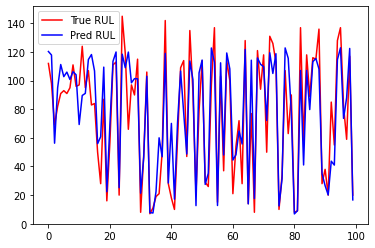
\includegraphics[width=\textwidth]{xgboost_cell30_out0.png}
\end{column}
\end{columns}
\end{frame}

\begin{frame}{Importance des variables -- XGBoost}
\begin{columns}[T]
\begin{column}{0.48\textwidth}
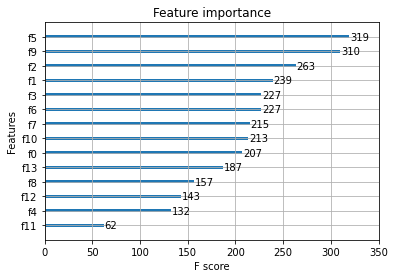
\includegraphics[width=\textwidth]{xgboost_cell32_out1.png}
\end{column}
\begin{column}{0.48\textwidth}
\textbf{Analyse :}
\begin{itemize}
    \item Certaines caractéristiques dominent la prédiction
    \item Les variables issues des capteurs de température et pression sont les plus informatives
    \item L'importance décroît rapidement après les 10 premières variables
\end{itemize}
\vspace{0.3cm}
\textbf{Limite :} le modèle ne capture pas explicitement la dimension temporelle.
\end{column}
\end{columns}
\end{frame}

% ==================== LSTM ====================
\section{Modèle LSTM}

\begin{frame}{Pourquoi les LSTM ?}
\begin{columns}[T]
\begin{column}{0.52\textwidth}
\textbf{Réseaux de Neurones Récurrents (RNN)}
\begin{itemize}
    \item Conçus pour les données séquentielles
    \item Maintiennent une mémoire interne de l'état passé
\end{itemize}
\vspace{0.3cm}
\textbf{LSTM (Long Short-Term Memory)}
\begin{itemize}
    \item Résolvent le problème de disparition du gradient
    \item Trois portes : oubli, entrée, sortie
    \item Capture des dépendances \textbf{long terme}
\end{itemize}
\vspace{0.3cm}
\textbf{Avantage pour CMAPSS :} la dégradation est un phénomène temporel étalé sur des centaines de cycles.
\end{column}
\begin{column}{0.44\textwidth}
\begin{block}{Architecture cellule LSTM}
\centering
\begin{tikzpicture}[scale=0.65, transform shape]
\node[draw, rectangle, fill=mainblue!20, minimum width=2cm, minimum height=1.2cm] (cell) at (0,0) {Cellule LSTM};
\node[draw, rectangle, fill=accentorange!30, minimum width=1.2cm] (forget) at (-2,1.5) {Oubli};
\node[draw, rectangle, fill=accentorange!30, minimum width=1.2cm] (input) at (0,1.5) {Entrée};
\node[draw, rectangle, fill=accentorange!30, minimum width=1.2cm] (output) at (2,1.5) {Sortie};
\draw[->, thick] (forget) -- (cell);
\draw[->, thick] (input) -- (cell);
\draw[->, thick] (output) -- (cell);
\node at (0,-0.8) {\small Portes : Oubli | Entrée | Sortie};
\end{tikzpicture}
\end{block}
\end{column}
\end{columns}
\end{frame}

\begin{frame}{Architecture du réseau LSTM implémenté}
\begin{center}
\begin{tikzpicture}[scale=0.75, transform shape,
    layer/.style={draw, rectangle, rounded corners, minimum width=3.5cm, minimum height=0.8cm, align=center, fill=mainblue!15},
    input/.style={draw, rectangle, fill=lightgray, minimum width=3cm, minimum height=0.7cm},
    output/.style={draw, rectangle, fill=accentorange!30, minimum width=2cm, minimum height=0.7cm}]

\node[input] (in) at (0,0) {Entrée $(30, 14)$};
\node[layer] (lstm1) at (0,-1.2) {LSTM -- 128 neurones\\tanh, return\_sequences};
\node[layer] (lstm2) at (0,-2.4) {LSTM -- 64 neurones\\tanh, return\_sequences};
\node[layer] (lstm3) at (0,-3.6) {LSTM -- 32 neurones\\tanh};
\node[layer] (dense1) at (0,-4.8) {Dense -- 96 neurones\\ReLU};
\node[layer] (dense2) at (0,-6.0) {Dense -- 128 neurones\\ReLU};
\node[output] (out) at (0,-7.2) {Sortie : RUL (1)};

\draw[->, thick] (in) -- (lstm1);
\draw[->, thick] (lstm1) -- (lstm2);
\draw[->, thick] (lstm2) -- (lstm3);
\draw[->, thick] (lstm3) -- (dense1);
\draw[->, thick] (dense1) -- (dense2);
\draw[->, thick] (dense2) -- (out);

\node[right=0.5cm of lstm1, align=left, font=\small] {\textbf{Paramètres :} 223~521};
\end{tikzpicture}
\end{center}
\end{frame}

\begin{frame}{Protocole d'entraînement}
\begin{columns}[T]
\begin{column}{0.48\textwidth}
\textbf{Optimiseur :} Adam
\begin{itemize}
    \item Taux initial : $10^{-3}$
    \item Réduction à $10^{-4}$ après 5 époques
\end{itemize}
\vspace{0.2cm}
\textbf{Partition :}
\begin{itemize}
    \item Train : 80\%
    \item Validation : 20\%
\end{itemize}
\vspace{0.2cm}
\textbf{Configuration :}
\begin{itemize}
    \item 10 époques
    \item Batch size : 128
    \item Perte : MSE
\end{itemize}
\end{column}
\begin{column}{0.50\textwidth}
\begin{block}{Évolution de la perte}
\centering
\small
\begin{tabular}{ccc}
\toprule
\textbf{Époque} & \textbf{Train} & \textbf{Val} \\
\midrule
1 & 3235 & 959 \\
5 & 210 & 169 \\
10 & 154 & \textbf{150} \\
\bottomrule
\end{tabular}
\end{block}
\vspace{0.2cm}
\textbf{Constat :} L'entraînement est volontairement court (10 époques) pour éviter le surapprentissage sur le jeu de validation.
\end{column}
\end{columns}
\end{frame}

\begin{frame}{Résultats LSTM sur FD001}
\begin{columns}[T]
\begin{column}{0.50\textwidth}
\begin{block}{Performances}
\centering
\begin{tabular}{lc}
\toprule
\textbf{Métrique} & \textbf{Valeur} \\
\midrule
RMSE & \textbf{15.17} cycles \\
S-score & \textbf{448.44} \\
\bottomrule
\end{tabular}
\end{block}
\vspace{0.3cm}
\textbf{Constats :}
\begin{itemize}
    \item Très bonne adéquation à la RUL réelle
    \item S-score très inférieur à XGBoost
    \item Moins de surestimations coûteuses
\end{itemize}
\end{column}
\begin{column}{0.48\textwidth}
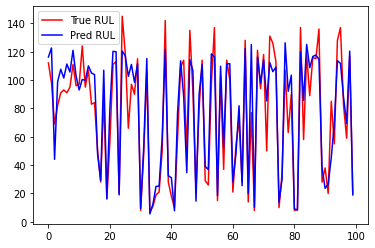
\includegraphics[width=\textwidth]{lstm_cell28_out0.png}
\end{column}
\end{columns}
\end{frame}

% ==================== COMPARAISON ====================
\section{Comparaison et discussion}

\begin{frame}{Tableau comparatif XGBoost vs LSTM}
\begin{center}
\begin{tabular}{lcc}
\toprule
\textbf{Métrique} & \textbf{XGBoost} & \textbf{LSTM} \\
\midrule
RMSE (cycles) & 19.07 & \textbf{15.17} \\
S-score & 1~024.43 & \textbf{448.44} \\
Nombre de paramètres & -- & 223~521 \\
Temps d'entraînement & Quelques secondes & $\sim$100 secondes \\
Capacité temporelle & \textcolor{accentorange}{Non} & \textcolor{mainblue}{Oui} \\
Interprétabilité & \textcolor{mainblue}{Élevée} & \textcolor{accentorange}{Faible} \\
\bottomrule
\end{tabular}
\end{center}
\vspace{0.3cm}
\begin{block}{Synthèse}
Le LSTM surpasse XGBoost de \textbf{20,4\%} en RMSE et divise le S-score par plus de 2, grâce à sa capacité à modéliser les dépendances temporelles.
\end{block}
\end{frame}

\begin{frame}{Discussion}
\begin{columns}[T]
\begin{column}{0.48\textwidth}
\begin{block}{Avantages LSTM}
\begin{itemize}
    \item Meilleure précision de prédiction
    \item Modélisation explicite du temps
    \item Moins de surestimations (S-score faible)
\end{itemize}
\end{block}
\end{column}
\begin{column}{0.48\textwidth}
\begin{alertblock}{Limites}
\begin{itemize}
    \item Complexité accrue (220k+ paramètres)
    \item Temps d'entraînement plus long
    \item Non-déterminisme des opérations GPU
    \item Faible interprétabilité (boîte noire)
\end{itemize}
\end{alertblock}
\end{column}
\end{columns}
\vspace{0.4cm}
\textbf{Reproductibilité :} Les poids du modèle pré-entraîné sont archivés (\texttt{.h5}) pour garantir des résultats identiques.
\end{frame}

% ==================== STREAMLIT ====================
\section{Démonstration Streamlit}

\begin{frame}{Application de démonstration}
\begin{columns}[T]
\begin{column}{0.52\textwidth}
\textbf{Objectif :} Mettre à disposition un outil interactif de prédiction de RUL.
\vspace{0.3cm}

\textbf{Fonctionnalités :}
\begin{itemize}
    \item Sélection d'un moteur parmi les 100 tests
    \item Visualisation des signaux capteurs
    \item Prédiction temps réel avec le modèle LSTM
    \item Affichage des métriques (RMSE, S-score)
    \item Comparaison True RUL vs Pred RUL interactive
\end{itemize}
\vspace{0.3cm}
\textbf{Technologies :} Streamlit, TensorFlow, Pandas, Plotly
\end{column}
\begin{column}{0.46\textwidth}
\begin{block}{Architecture}
\centering
\begin{tikzpicture}[scale=0.6, transform shape,
    box/.style={draw, rectangle, rounded corners, fill=mainblue!15, minimum width=2.5cm, minimum height=0.7cm, align=center, font=\small}]
\node[box] (data) at (0,0) {Données\\CMAPSS};
\node[box] (prepro) at (0,-1.5) {Prétraitement\\Pipeline};
\node[box] (model) at (0,-3) {Modèle LSTM\\(.h5)};
\node[box] (app) at (0,-4.5) {Interface\\Streamlit};
\draw[->, thick] (data) -- (prepro);
\draw[->, thick] (prepro) -- (model);
\draw[->, thick] (model) -- (app);
\end{tikzpicture}
\end{block}
\end{column}
\end{columns}
\end{frame}

% ==================== CONCLUSION ====================
\section{Conclusion}

\begin{frame}{Conclusion}
\textbf{Réalisations :}
\begin{enumerate}
    \item Pipeline complet de prétraitement des données CMAPSS
    \item Implémentation et comparaison de XGBoost et LSTM
    \item Supériorité du LSTM (RMSE 15.17 vs 19.07 cycles)
    \item Application Streamlit de démonstration
\end{enumerate}
\vspace{0.3cm}
\textbf{Perspectives :}
\begin{itemize}
    \item Extension aux sous-ensembles FD002, FD003, FD004
    \item Intégration de mécanismes d'attention (GRU + Attention)
    \item Prédiction probabiliste (distribution de RUL)
    \item Déploiement embarqué (quantification, pruning)
\end{itemize}
\end{frame}

\begin{frame}
\begin{center}
{\Huge \textbf{Merci de votre attention}}
\vspace{1cm}

{\Large Questions ?}
\vspace{1.5cm}

\textbf{Contact :} [votre.email@ecole.fr]

\vspace{0.5cm}
\small
\textit{Code source :} \url{https://biswajitsahoo1111.github.io/rul_codes_open/}
\end{center}
\end{frame}

\end{document}
